\documentclass[11pt]{article}

\usepackage[margin=1in]{geometry}
\usepackage{amsmath,amssymb}
\usepackage{booktabs}
\usepackage{tabularx}
\usepackage{enumitem}
\usepackage{microtype}
\usepackage{graphicx}
\setlist{nosep,leftmargin=*}

\newcommand{\code}[1]{\texttt{#1}}
\newcommand{\Gt}{\Gamma_t}
\newcommand{\alphas}{\alpha_s}
\newcommand{\cE}{\mathcal{E}}
\newcommand{\JKT}{[JKT]}
\newcommand{\Fuks}{[Fuks]}
\newcommand{\Vh}{\hat V}
\newcommand{\qc}{q_\mathrm{cut}}
\newcommand{\As}{\mathcal{A}}
\newcommand{\MS}{\overline{\mathrm{MS}}}
\newcommand{\fn}[1]{\hfill$\to$~\code{#1}}
\newcolumntype{L}{>{\raggedright\arraybackslash}X}

\title{Solving for the toponium Green's function with the method of Je\.zabek, K\"uhn and Teubner}
\author{Artemiy}
\date{\today}

\begin{document}
\maketitle

\begin{abstract}
\noindent Artemiy's funky attempt at toponium. Near threshold, everything about a $t\bar t$ pair that feels the QCD
potential is contained in one complex function, the S-wave Green's function $G(E,p)$. This note shows how I compute it
from scratch by following \JKT\ equation by equation: the potential of their Sec.~2, the regularisation and numerical
solution of their Sec.~3, the checks that the solver is right, and what it gives when used to re-weight MadGraph events.
Fuks et al.\ appear only as the point of comparison: they publish tables of $G$, but not how they made them.
\end{abstract}

\noindent\textbf{References} (PDFs in \code{reference/})
\begin{itemize}
  \item \JKT\ M.~Je\.zabek, J.H.~K\"uhn, T.~Teubner, Z.~Phys.~C 56 (1992) 653 (\code{BF01474740.pdf}). \emph{The method.}
  \item \Fuks\ B.~Fuks, K.~Hagiwara, K.~Ma, Y.-J.~Zheng, arXiv:2411.18962v2 (\code{2411.18962v2.pdf}). \emph{The comparison.}
\end{itemize}
Equation numbers always refer to the paper named in front of them: \JKT\ (21) is Eq.~(21) of JKT.
The code is one library, \code{toponium.py}; a ``$\to$~\code{name}'' at the end of a paragraph names the class or method
that implements it.

%==========================================================================================
\section{The problem}

A $t\bar t$ pair produced at a point with energy $E=W-2m_t$ ($W$ the pair's invariant mass) and relative momentum $p$
propagates as
\begin{gather*}
G(\vec p,E)=\int d^3r\,e^{i\vec p\cdot\vec r}\,G(\vec r,0;E)
=\Big\langle\vec p\,\Big|\frac{1}{\cE-H}\Big|\,\vec r=0\Big\rangle,\\
H=\frac{p^2}{m_t}+V(r),\qquad \cE=E+i\Gt
\qquad\text{(\JKT\ (2)--(4))}.
\end{gather*}
The width enters through $E\to\cE$: the tops decay before the pair can form a stable bound state, so the toponium
``resonances'' are smeared into a single bump. Without the potential,
$$
G_0(p)=\frac{1}{\cE-p^2/m_t}\qquad\text{(\JKT\ (6))},
$$
and the potential's whole effect is in the ratio $G/G_0$. In particular, re-weighting each MadGraph $t\bar t$ event by
$|G(E,p^*)/G_0(E,p^*)|^2$ (\Fuks\ (15)) puts toponium into the event sample.

So the task is: \emph{compute $G(E,p)$ for the QCD potential.} \JKT\ give both the potential (their Sec.~2) and a numerical
method (their Sec.~3), and I follow both as printed. Where they leave a choice open, I say so and list it in
Sec.~\ref{sec:departures}.

\paragraph{Contrast with Fuks et al.}
\Fuks\ use the same re-weighting but do not say how they computed $G$; they publish it as a table (swData) and cite
\JKT. My $G$ is computed independently of those tables. Comparing the two turned out to be a test of the tables rather than
of my solver (Sec.~\ref{sec:fuks}).

Conventions: $m_t=173$~GeV, $\Gt=1.49$~GeV, $C_F=4/3$, $n_F=5$, $\alphas(m_Z)=0.12$. $G$ has the sign of \JKT\ (6).
\fn{Constants, Constants.G0}

%==========================================================================================
\section{The method at a glance}

\begin{center}\small
\begin{tabularx}{\linewidth}{@{}l l L@{}}
\toprule
\JKT\ & what it is & in \code{toponium.py} \\
\midrule
(14) & two-loop running coupling $\alphas(Q^2)$ & \code{JKTPotential.alpha\_2loop}, \code{lambda\_msbar\_2loop}\\
(13) & perturbative potential $\tilde V_\mathrm{pert}(Q^2)$ & \code{JKTPotential.V\_pert}\\
(15) & full potential: (13) above 5~GeV, Richardson-like below & \code{V\_ir}, \code{continuity\_constant\_C}, \code{V\_jkt}\\
(19)--(20) & cut at small momentum, and its normalisation & \code{V\_cut}, \code{V\_cut\_position}, \code{energy\_shift}\\
(16)--(17) & $G=G_0K$ and the integral equation for $K$ & \code{LSSolver.G}\\
(18) & S-wave kernel $\Vh(p,q)$ & \code{LSSolver.kernel}\\
(21)--(22) & subtracted equation and $\As(p)$ & \code{LSSolver.script\_A}, \code{solve\_K}\\
(23) & Gauss--Legendre grid & \code{LSSolver.jkt\_grid}\\
\bottomrule
\end{tabularx}
\end{center}

\medskip
\noindent\fbox{\begin{minipage}{\dimexpr\linewidth-2\fboxsep-2\fboxrule}\small
\textbf{Algorithm.} Input: $\alphas(m_Z)$, $m_t$, $\Gt$.
\begin{enumerate}[label=\arabic*.]
\item Build the potential: $\Lambda_{\MS}$ from (14) at $m_Z$, then (13), (15), the cut (19). \hfill Sec.~\ref{sec:potential}
\item Fix the cut's $\delta^3$ term by (20); it becomes a constant energy shift. \hfill Sec.~\ref{sec:cut}
\item Tabulate $F(s)=\int_0^sV\,dk^2$, which gives the kernel (18). \hfill Step 2
\item Nodes and weights $q_j,w_j$ (23); matrix $W_{ij}=w_j\Vh(q_i,q_j)$, zero diagonal. \hfill Steps 2, 5
\item For each $E$: $g_j=G_0(q_j;E-\text{shift})$, $\As(q_i)$ (22), solve (21) for $K_i$. \hfill Steps 3, 4, 6
\item For each output $p$: $G(p)=G_0(p)\,K(p)$ (16), $K$ splined between nodes. \hfill Step 7
\end{enumerate}
\end{minipage}}

%==========================================================================================
\section{The potential (JKT Sec.~2 and the cut of Sec.~3)}
\label{sec:potential}

Everything here is in momentum space: $\tilde V(Q^2)$, with $Q$ the momentum transfer. \fn{JKTPotential}

\paragraph{The running coupling, \JKT\ (14).}
$$
\alpha_{\MS}(Q^2)=\frac{4\pi}{b_0\ln\!\big(Q^2/\Lambda_{\MS}^2\big)+\dfrac{b_1}{b_0}\ln\ln\!\big(Q^2/\Lambda_{\MS}^2\big)},
\qquad b_0=11-\tfrac23n_F,\quad b_1=102-\tfrac{38}{3}n_F .
$$
JKT quote $\alphas$ directly; I quote $\alphas(m_Z)=0.12$, the value \Fuks\ use, and \emph{solve} (14) for $\Lambda$: with
$x=\ln(m_Z^2/\Lambda^2)$, (14) at $Q=m_Z$ reads
$$
b_0\,x+\frac{b_1}{b_0}\ln x=\frac{4\pi}{\alphas(m_Z)},
$$
a single equation in $x$, solved by root-finding (Brent's method). This is the only equation solved in building the
potential; everything after it is evaluated directly. For $\alphas(m_Z)=0.12$, $n_F=5$: $\Lambda_{\MS}^{(5)}=223$~MeV,
and (14) then gives $\alphas=0.221$, $0.183$, $0.157$, $0.150$ at $Q=5$, $10$, $20$, $25$~GeV.
\fn{beta\_coefficients, lambda\_msbar\_2loop, alpha\_2loop}

\paragraph{The perturbative potential, \JKT\ (13).}
$$
\tilde V_\mathrm{pert}(Q^2)=-\frac{16\pi}{3}\,\frac{\alpha_{\MS}(Q^2)}{Q^2}
\left[1+\left(\frac{31}{3}-\frac{10}{9}n_F\right)\frac{\alpha_{\MS}(Q^2)}{4\pi}\right].
$$
This is one-gluon exchange, $-4\pi C_F\alpha/Q^2$ with $4\pi C_F=16\pi/3$, with two improvements: the coupling runs with the
momentum transfer, $\mu^2=Q^2$, by (14), and the square bracket is the one-loop correction to the potential. Nothing is
solved: for each $Q^2$, compute $\alpha_{\MS}(Q^2)$ from (14), put it into (13). (With $\alpha$ held fixed this is the
potential of \Fuks\ (12); without the bracket and with fixed $\alpha$ it is plain Coulomb, the test case of
Sec.~\ref{sec:coulomb}.)
\fn{V\_pert}

\paragraph{Joining to the long-distance potential, \JKT\ (15).}
(13) is valid only at large $Q$; at small $Q$ the coupling blows up at $Q=\Lambda$. Below $|\vec p|=5$~GeV JKT switch to a
Richardson-like form that also produces the linear confining potential:
$$
\tilde V(\vec p)=\begin{cases}\tilde V_\mathrm{pert}(p^2,n_F=5), & |\vec p|>5\text{ GeV},\\[4pt]
-\dfrac43\,\dfrac{48\pi^2}{27}\,\dfrac{1}{p^2}\left(\dfrac{1}{\ln(1+p^2/\Lambda_R^2)}+C\right), & |\vec p|<5\text{ GeV},\end{cases}
\qquad\Lambda_R=400\text{ MeV}.
$$
$C$ is fixed by continuity at 5~GeV: setting the two lines equal at $p^2=25$~GeV$^2$ and solving for $C$ (one linear
equation) gives $C=-0.0262$. At small $p$, $1/\ln(1+p^2/\Lambda_R^2)\approx\Lambda_R^2/p^2$, so
$\tilde V\approx-\kappa\Lambda_R^2/p^4$ with $\kappa=\tfrac43\cdot\tfrac{48\pi^2}{27}$: the Fourier transform of a potential
rising linearly with $r$.
\fn{V\_ir, continuity\_constant\_C, V\_jkt}

\paragraph{The cut, \JKT\ (19).}
\label{sec:cut}
The $1/p^4$ behaviour is a problem: its Fourier integral diverges at $p\to0$, and the kernel (18) built from it is singular as
$(p-q)^{-2}$ at $q=p$. JKT argue that $t$ and $\bar t$ decay before they reach the confining distances, so $G$ cannot depend on
how the potential behaves at very small momentum, and they replace it there:
$$
\tilde V_\mathrm{cut}(\vec p;\qc)=\begin{cases}\tilde V(\vec p), & |\vec p|>\qc,\\[2pt]
-\dfrac{C_1}{p^2+\qc^2}+\tilde V_0(\qc)\,\delta^3(\vec p), & |\vec p|<\qc,\end{cases}\qquad \qc=50\text{ MeV}.
$$
$C_1$ comes from continuity at $p=\qc$: $-C_1/(2\qc^2)=\tilde V(\qc^2)$.

\paragraph{Normalising the cut, \JKT\ (20).}
Cutting changes $V(r)$ by a constant. JKT fix $\tilde V_0$ by demanding that the position-space potential
$$
V_\mathrm{cut}(r;\qc)=\int\!\frac{d^3q}{(2\pi)^3}\,e^{-i\vec q\cdot\vec r}\,\tilde V_\mathrm{cut}(\vec q;\qc)
=\frac{1}{2\pi^2r}\int_0^\infty\!dq\,q\sin(qr)\,\tilde V_\mathrm{cut}(q^2)+\frac{\tilde V_0}{(2\pi)^3}
$$
satisfy $V_\mathrm{cut}(r=1\,\mathrm{GeV}^{-1})=-\tfrac14$~GeV. The $\delta^3$ term is just the constant
$\tilde V_0/(2\pi)^3$ in $V(r)$, i.e.\ a constant added to $H$, so in the Green's function it is the same as
$E\to E-\tilde V_0/(2\pi)^3$. I therefore solve with the smooth part of (19) and evaluate $G_0$ at the shifted energy.
For $\alphas(m_Z)=0.12$ the shift is $+5.678$~GeV. It is large because it cancels the constant $\sim\kappa\Lambda_R^2/(2\pi^2\qc)$
that the cut adds to $V(r)$; it depends on $\qc$, but $G$ does not (Sec.~\ref{sec:checks}).
\fn{V\_cut, V\_cut\_position, energy\_shift}

%==========================================================================================
\section{Solving the Lippmann--Schwinger equation (JKT Sec.~3)}
\label{sec:solver}

\paragraph{Step 1: the equation, \JKT\ (5), (16)--(17).}
The Green's function obeys
$$
G(\vec p)=G_0(p)+G_0(p)\int\!\frac{d^3q}{(2\pi)^3}\,\tilde V(\vec p-\vec q)\,G(\vec q)\qquad\text{(\JKT\ (5))}.
$$
For the S-wave JKT write $G=G_0K$ (16), and the vertex function $K$ obeys
$$
K(p)=1+\int_0^\infty\!dq\,\Vh(p,q)\,G_0(q)\,K(q)\qquad\text{(\JKT\ (17))}.
$$
$K$ is smooth in $p$: the sharp structure of $G$ (the on-shell peak at $p^2=m_tE$ for $E>0$) sits in $G_0$, which is known exactly.

\paragraph{Step 2: the S-wave kernel, \JKT\ (18).}
The angular integral of $\tilde V(|\vec p-\vec q|)$ gives
\begin{gather*}
\Vh(p,q)=\frac{1}{4\pi^2}\frac qp\int_{|p-q|}^{p+q}\!du\,u\,\tilde V(u)=\frac{q}{8\pi^2p}\Big[F\big((p+q)^2\big)-F\big((p-q)^2\big)\Big],\\
F(s)=\int_0^s\!dk^2\,\tilde V(k^2).
\end{gather*}
$F$ is computed once per potential (10-point Gauss--Legendre on 6000 cells in $\ln s$, with the kinks of $\tilde V$ at $\qc$ and
5~GeV on cell edges) and splined. This is the only place the potential of Sec.~\ref{sec:potential} enters the solver. For pure
Coulomb, $\tilde V=-B/k^2$, the integral is elementary: $\Vh=-\frac{Bq}{8\pi^2p}\ln\frac{(p+q)^2}{(p-q)^2}$.
\fn{LSSolver.kernel}

\paragraph{Step 3: the peak at $q=p$, and JKT's subtraction, \JKT\ (21)--(22).}
$\Vh(p,q)$ is large at $q=p$ (small momentum transfer). With the cut it is finite but peaked on the scale $\qc=50$~MeV; for Coulomb it
has a logarithmic singularity. The grid nodes (Step~5) are $\sim0.1$--$0.25$~GeV apart, so a plain Gauss--Legendre sum misses the
peak (Fig.~\ref{fig:kernel}, left).

Why not simply put more nodes there? Because ``there'' is everywhere: the same nodes $q_j$ serve every row $p=q_i$ of the
linear system (Step~6), and the peak of row $i$ sits at $q=q_i$, on a node of its own. Refining the grid around one $p$ does
nothing for the others; resolving a 50~MeV peak at every node would take a grid $\sim$100 times finer, $N\sim10^4$. JKT
instead add and subtract $K(p)$ inside the integral of (17):
\begin{align*}
\big[1-\As(p)\big]K(p)+\int_0^\infty\!dq\,\Vh(p,q)\,G_0(q)\,\big[K(p)-K(q)\big]&=1, &&\text{(\JKT\ (21))}\\
\As(p)=\int_0^\infty\!dq\,\Vh(p,q)\,G_0(q)&. &&\text{(\JKT\ (22))}
\end{align*}
This is an identity, not an approximation. It moves the peak into $\As(p)$, which contains no unknown: in JKT's words, ``a known
function which can be evaluated by a numerical integration''. In the remaining integral the peak is multiplied by
$K(p)-K(q)\approx K'(p)(p-q)$, which vanishes at $q=p$. What is left is $\sim1000$ times smaller and odd about $q=p$, so the
contributions of the nodes on either side largely cancel (Fig.~\ref{fig:kernel}, right). The peak is then integrated
\emph{once per $p$}, in $\As(p)$, where a fine rule built around that one $p$ is cheap (Step~4, Fig.~\ref{fig:kernel}, middle).

\begin{figure}[h]
\centering
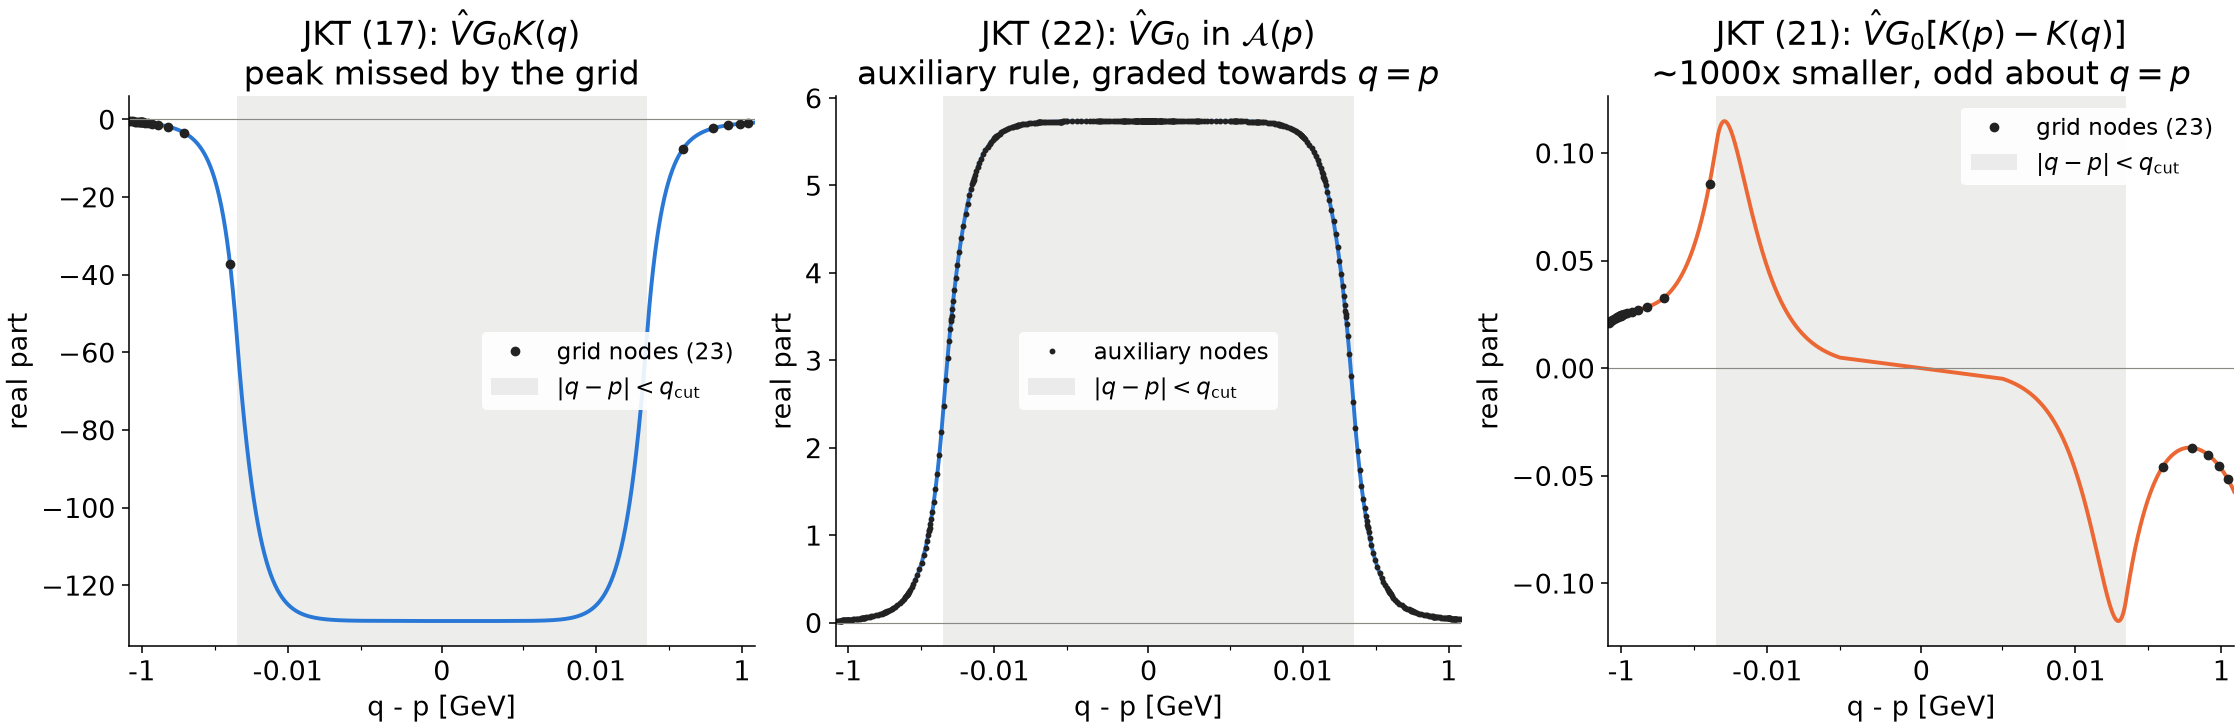
\includegraphics[width=\linewidth]{results/0_solver_checks/kernel_subtraction.png}
\caption{JKT potential ($\alphas(m_Z)=0.12$, $\qc=50$~MeV), $p=5$~GeV, $E=-2$~GeV, against $q-p$ on a logarithmic scale
(linear for $|q-p|<1$~MeV) so that the peak region, $|q-p|\lesssim\qc$ (shaded), is spread out. Left: the integrand of \JKT\ (17)
with the grid nodes of \JKT\ (23): the peak lies between two nodes. Middle: the integrand of \JKT\ (22), on the auxiliary rule of
$\As(p)$, whose panels are graded geometrically towards $q=p$ and so are evenly spaced on this axis. Right: the integrand of
\JKT\ (21), $\sim1000\times$ smaller and odd about $q=p$, which the grid nodes integrate accurately.}
\label{fig:kernel}
\end{figure}

\paragraph{Step 4: computing $\As(p)$, \JKT\ (22).}
JKT do not say how. I use a fine auxiliary Gauss--Legendre rule for each $p$: 16-point panels with edges graded geometrically towards
$q=p$ ($p(1\pm2^{-k})$, $k\le24$, i.e.\ evenly spaced in $\ln|q-p|$; Fig.~\ref{fig:kernel}, middle) to resolve the peak, further edges at $p(1+2^k)$ for its fall-off, every 2~GeV up to 200~GeV for the
on-shell peak of $G_0$, and a $t=1/q$ tail. $\Vh$ on these points is stored once, so for each energy $\As(p)$ is one dot product with
$G_0$. Against adaptive quadrature the relative error is $2\times10^{-10}$ (Coulomb) and $6\times10^{-6}$ (JKT, limited by the spline
of $F$).
\fn{LSSolver.aux\_rule, script\_A}

\paragraph{Step 5: the grid, \JKT\ (23).}
Every $\int_0^\infty dq$ in (21) becomes a Gauss--Legendre sum $\sum_jw_j(\cdot)(q_j)$. JKT use three subintervals, $(0,a_1)$,
$(a_1,a_2)$ and $(0,1/a_2)$ in $t=1/q$, with $a_1\sim\sqrt{m_t\Gt}$ and $a_2\sim m_t$. I split them once more, at 4 and 60~GeV:
edges $0,4,16,60,m_t$ plus the $t=1/q$ tail, with $n=48$ points each ($N=240$; JKT used $N=100$--$400$). The reason: above
threshold at narrow width ($m_t=120$, $\Gt=0.3$~GeV, JKT's Fig.~4a at $E=2$), the on-shell peak of $G_0$ at $p_0=\sqrt{m_tE}$
is only $m_t\Gt/2p_0\approx1.2$~GeV wide. On JKT's wide middle panel it falls between the nodes, and the peak of $|pG|^2$ goes
$9272\to7680\to7219$ for $n=48,96,160$ without settling. With the extra breaks it gives $7065,7044,7036$ (JKT: $\sim7050$).
\fn{LSSolver.jkt\_grid}

\paragraph{Step 6: one linear system per energy.}
Imposing (21) at the nodes $p=q_i$ gives, with $g_j=G_0(q_j)$ and $W_{ij}=w_j\Vh(q_i,q_j)$,
$$
\Big[1-\As(q_i)+\sum_{j\ne i}W_{ij}g_j\Big]K_i-\sum_{j\ne i}W_{ij}g_jK_j=1 .
$$
The $j=i$ term drops out exactly, because it multiplies $K_i-K_i=0$. $W$ does not depend on $E$ and is built once. Each energy costs
$\As$ (Step~4) and one dense $N\times N$ solve.
\fn{LSSolver.solve\_K}

\paragraph{Step 7: $G$ at any $p$, \JKT\ (16).}
$G(p)=G_0(p)K(p)$, with $K$ between the nodes from a cubic spline in $\ln q$ through the $K(q_i)$. Because $K$ is smooth and $G_0$ is exact,
this keeps the sharp structure of $G$. (I also tried evaluating (21) itself at off-grid $p$. That is 10--40 times less accurate,
because at a general $p$ the nodes are not placed symmetrically around the peak of Step~3.)
\fn{LSSolver.G}

%==========================================================================================
\section{Is the solver right?}
\label{sec:checks}

\subsection{Ground truth: the exact Coulomb solution}
\label{sec:coulomb}
For a fixed-coupling Coulomb potential, $V=-C_F\alpha/r$, the equation can be solved on paper (JKT mention this below their (12)).
The solution is a Whittaker function,
$$
G(r)=-\frac{m_t}{4\pi r}\,\Gamma(1-\lambda)\,W_{\lambda,1/2}(2\kappa r),\qquad \kappa=\sqrt{-m_t\cE},\quad \lambda=\frac{C_F\alpha m_t}{2\kappa},
$$
and its Laplace representation plus the S-wave Fourier transform give a one-dimensional integral,
$$
\tilde G(p)=-4m_t\kappa^2\!\int_0^\infty\!dt\,\frac{t^{-\lambda}(1+t)^{\lambda}(1+2t)}{\big(\kappa^2(1+2t)^2+p^2\big)^2},
$$
which is $G_0$ at $\lambda\to0$. It converges at $t\to0$ only for $\mathrm{Re}\,\lambda<1$ ($\lambda=1$ is the 1S pole), so it is
continued by subtracting $f(0)$ on $[0,1]$, valid for $\mathrm{Re}\,\lambda<2$; since $|\lambda|\le1.08$ for $\alpha=0.15$, one
subtraction suffices. No numerical solver is involved.
\fn{CoulombExact}

\subsection{Accuracy and $\qc$ independence (Stage 0)}
On $E\in[-6,4]$~GeV, $p\in[0.5,29.5]$~GeV, $m_t=173$, $\Gt=1.49$~GeV. The solver with a Coulomb potential is compared with the exact
solution; with the JKT potential, against itself at $n=96$:

\begin{center}\small
\begin{tabular}{@{}rrcccc@{}}
\toprule
 & & \multicolumn{2}{c}{Coulomb $\alpha=0.15$ vs exact} & \multicolumn{2}{c}{JKT $\alphas(m_Z)=0.12$ vs $n=96$}\\
\cmidrule(lr){3-4}\cmidrule(l){5-6}
$n$ & $N$ & median & max & median & max\\
\midrule
16 & 80  & $5.3\times10^{-5}$ & $1.1\times10^{-2}$ & $6.5\times10^{-4}$ & $8.9\times10^{-2}$\\
24 & 120 & $1.4\times10^{-5}$ & $2.2\times10^{-3}$ & $2.4\times10^{-4}$ & $2.1\times10^{-2}$\\
32 & 160 & $5.9\times10^{-6}$ & $7.0\times10^{-4}$ & $1.2\times10^{-4}$ & $8.9\times10^{-3}$\\
48 & 240 & $1.8\times10^{-6}$ & $2.0\times10^{-4}$ & $5.4\times10^{-5}$ & $3.2\times10^{-3}$\\
64 & 320 & $7.5\times10^{-7}$ & $8.0\times10^{-5}$ & $2.5\times10^{-5}$ & $1.4\times10^{-3}$\\
\bottomrule
\end{tabular}
\end{center}
The maxima sit above threshold on the on-shell ridge; for $E\le0$ they are $1.1\times10^{-5}$ (Coulomb) and $5.8\times10^{-4}$ (JKT) at
$n=48$. JKT quote ``better than 1\%, typically $10^{-3}$''.

\emph{$\qc$ independence} (JKT: ``$K$ is independent from $\qc$ for $\qc<200$~MeV''). Relative to $\qc=50$~MeV, $G$ changes by at most
$4.9\times10^{-3}$ at 200~MeV, $1.6\times10^{-3}$ at 100~MeV, $1.0\times10^{-3}$ at 20~MeV and $1.3\times10^{-3}$ at 10~MeV, while the energy
shift of (20) ranges from $1.6$ to $27$~GeV. The cut does what JKT claim: it regularises without changing the physics.

\subsection{Reproducing JKT's own results (Stage 1)}
Since this is JKT's method, it must reproduce their figures (Fig.~\ref{fig:jkt}). I use $\alphas=0.125$ as JKT do, and $\Gt$ from \JKT\ (8)--(9): $0.299$,
$0.807$ and $1.563$~GeV for $m_t=120$, $150$ and $180$ (JKT's text rounds to $0.3/0.8/1.5$). At $m_t=120$ the 1S peak of $R$ is at
$-2.32$~GeV (JKT: $-2.3$) with height $3.80$ (JKT: $3.78$). The 1S--2S minimum, the 2S bump, $R(0)$ and $R(4)$ agree to $0.2$--$2\%$.
The peaks of $|pG|^2$ in their Fig.~4a--c agree to $0$--$3\%$ with the values read off by eye, and $-G(p\to0)$ in their Fig.~2 to
$0.4$--$3\%$. The exception is $\mathrm{Im}(-G)(p\to0)$ at $E=0$ (Fig.~3): $-2.98$ against their $-2.7$, i.e.\ $10\%$, on a small value
on a $\pm8$ axis. The optical theorem \JKT\ (12), $\int\!\frac{d^3p}{(2\pi)^3}\Gt|G|^2=-\mathrm{Im}\,G(0,0)$, holds to $4\times10^{-5}$
for $E\in[-5,5]$~GeV; it is not built into the solver, so it independently checks the solution.

\begin{figure}[htbp]
\centering
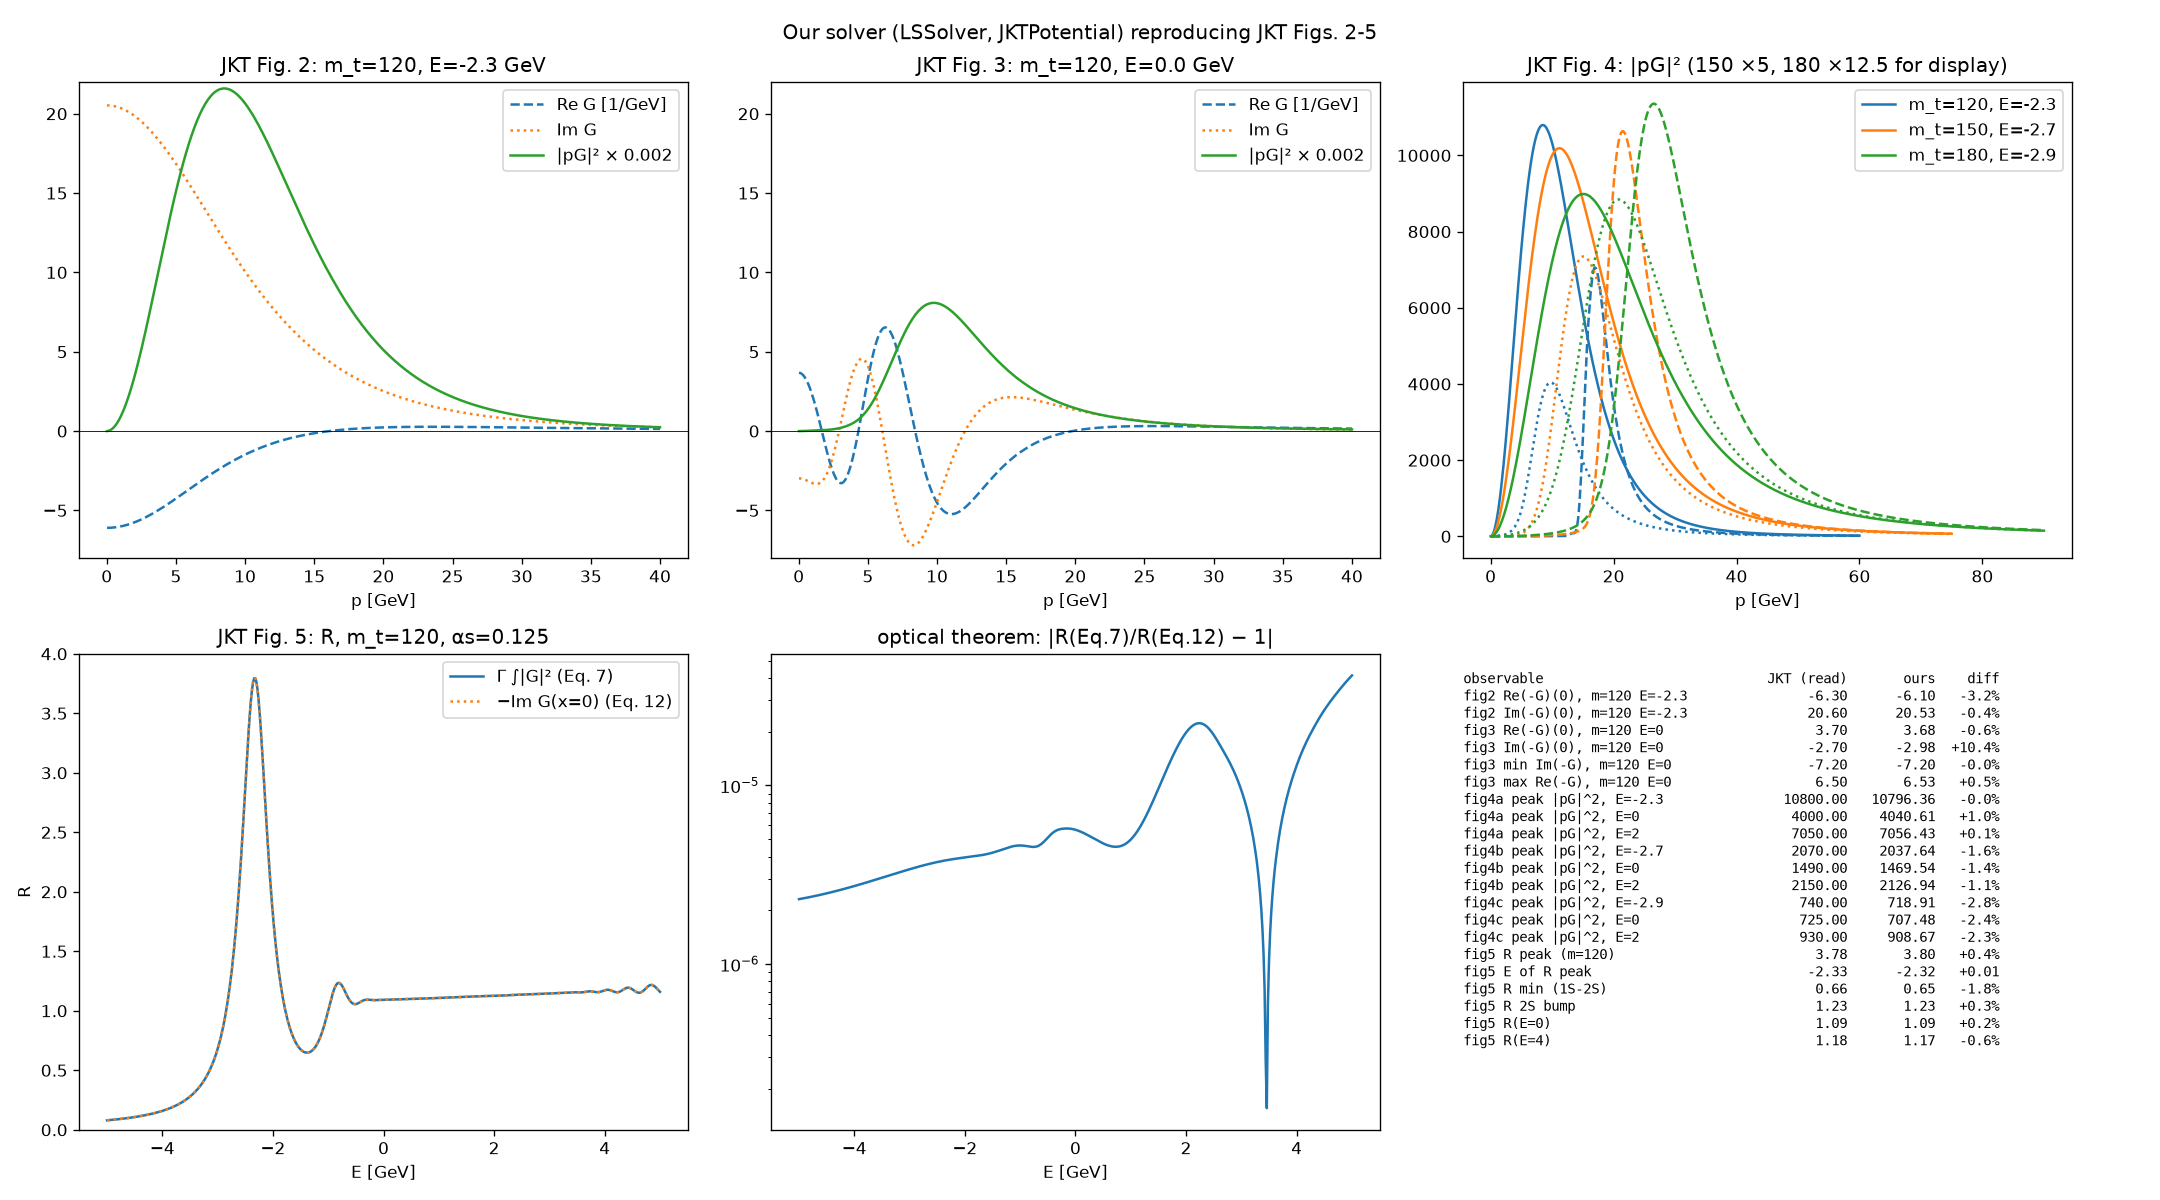
\includegraphics[width=\linewidth]{results/1_validate_jkt/jkt_figs.png}
\caption{JKT's Figs.~2--5 recomputed with my solver ($\alphas=0.125$, $\Gt$ from \JKT\ (8)). Top: $G$ and $|pG|^2$ at
$m_t=120$~GeV at the 1S peak and at threshold; $|pG|^2$ for $m_t=120,150,180$~GeV (solid, dotted, dashed: below, at and
above threshold). Bottom: the cross-section ratio $R(E)$ from $\int\Gt|G|^2$ and from $-\mathrm{Im}\,G(0,0)$ (the optical
theorem \JKT\ (12)), their relative difference, and the comparison with values read off JKT's figures.
(\code{1\_validate\_jkt.py})}
\label{fig:jkt}
\end{figure}

One convention to watch: JKT's Figs.~1--3 plot $-G$ relative to their (6) and (10). At the 1S peak their Fig.~2 has
$\mathrm{Im}\approx+20$~GeV$^{-1}$ at $p\to0$, whereas $\mathrm{Im}\,G=-|\psi(0)|^2/\Gt<0$.

%==========================================================================================
\section{Using it for toponium, and the contrast with Fuks et al.}
\label{sec:fuks}

\paragraph{What Fuks et al.\ do.} They re-weight colour-singlet $gg\to t\bar t\to b\ell^+\nu\,\bar b\ell'^-\bar\nu$ MadGraph events by
$|G/G_0|^2$ (\Fuks\ (15)), with $G$ interpolated from their swData tables by their Fortran routine \code{CALCGREEN}. They describe the
potential behind the tables in four different ways (running tree-level coupling, Richardson following \JKT, fixed
$\alphas(m_Z)=0.12$, two-loop) and do not describe the method. I read their tables and run their routine exactly as published, as a
reference to compare with. \fn{FuksTables}

\paragraph{What is in their tables (Stage 2).} Fitting each of their descriptions to swData, using my solver and the exact Coulomb
solution (rms of $|\text{swData}/\text{model}-1|$ on $E\in[-6,4]$, $p<30$~GeV):

\begin{center}\small
\begin{tabularx}{\linewidth}{@{}Lr@{}}
\toprule
Potential & rms\\
\midrule
fixed-$\alpha$ tree Coulomb, best fit $\alpha=0.1500$, $m_t=172.96$, $\Gt=1.4907$ & $0.13\%$\\
fixed $\alpha=0.12$ (their Fig.~1 caption), with or without the bracket of (13) & 40--50\%\\
JKT potential (13)--(15), $\alphas(m_Z)=0.12$, tree or NLO & 55--69\%\\
\quad the same, with a free energy offset & 15--17\%\\
\bottomrule
\end{tabularx}
\end{center}

\noindent So swData is the exact fixed-coupling Coulomb Green's function at $\alpha=0.15$, not the JKT potential. A plausible origin:
$\alphas(m_Z)=0.12$ run with (14) reaches $0.150$ at $Q\approx25$~GeV, close to the Bohr momentum (Sec.~\ref{sec:potential}). The
authors state neither. My solver with Coulomb $\alpha=0.15$ reproduces their tables as well as the exact solution does (median
deviation $2.6\times10^{-3}$ for both, Stage 3, Fig.~\ref{fig:fuks1}), which is a further check of the solver.

\begin{figure}[htbp]
\centering
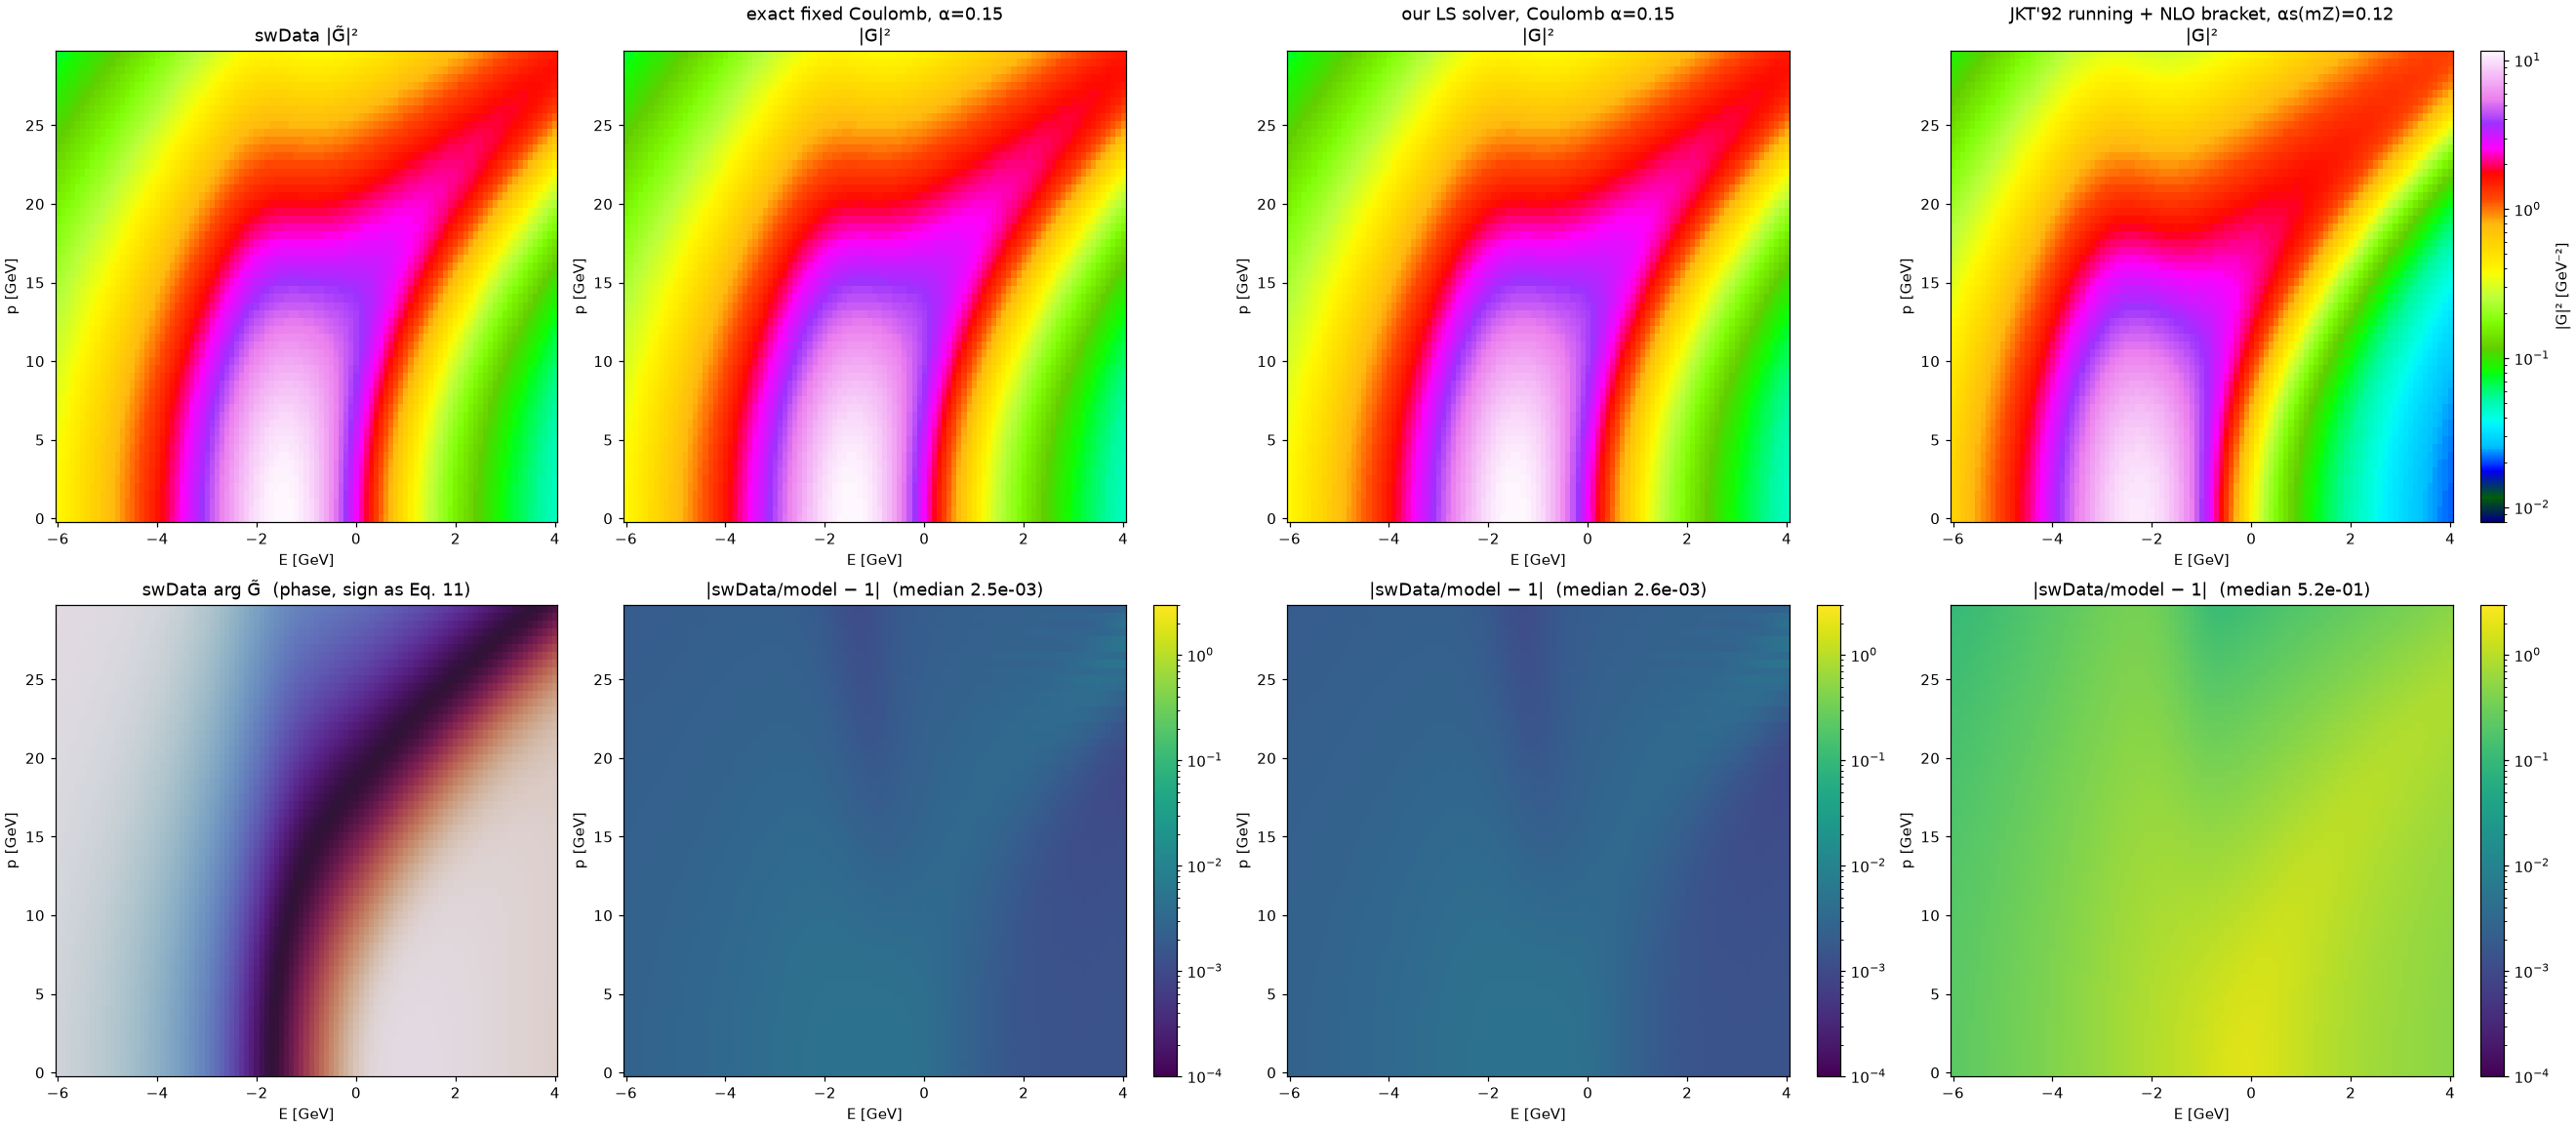
\includegraphics[width=\linewidth]{results/3_fuks_fig1/fig1_ours_vs_swdata.png}
\caption{Fuks's Fig.~1, rebuilt from their swData (left column: $|\tilde G|^2$ and phase), next to exact Coulomb at
$\alpha=0.15$, my solver with Coulomb at $\alpha=0.15$, and my solver with the JKT potential at $\alphas(m_Z)=0.12$.
Bottom row: $|\text{swData}/\text{model}-1|$. (\code{3\_fuks\_fig1.py})}
\label{fig:fuks1}
\end{figure}

\paragraph{Events (Stage 4).} 13 TeV, CT18NLO, $m_t=173$, $\Gt=1.49$: 500k colour-singlet ($330\le W\le350$~GeV, colour matrix
\Fuks\ (20)) and 500k full colour ($340\le W\le350$); the window is imposed by restricting $\tau=\hat s/s$ in MadGraph's \code{genps.f}.
The singlet fraction is 0.281 (expected $2/7$). The same events are re-weighted with three sources of $G$:

\begin{center}\small
\begin{tabular}{@{}lccc@{}}
\toprule
 & Fuks: swData & Coulomb $\alpha=0.15$ & \textbf{JKT potential (this note)}\\
 & via \code{CALCGREEN} & exact & $\alphas(m_Z)=0.12$\\
\midrule
$\sigma_\mathrm{rw}/\sigma$ ($p^*<50$~GeV) & 8.88 & 8.90 & 7.89\\
$\langle p^*\rangle(E=-2)$ [GeV] & 20.7 & 20.7 & 19.6\\
peak of $d\sigma/dW$ [GeV] & 344.75 & 344.75 & 343.75\\
\bottomrule
\end{tabular}
\end{center}
With Fuks's own $G$ the re-weighted distributions reproduce their Figs.~2--5 (Figs.~\ref{fig:fuks2}--\ref{fig:fuks5}). The
JKT potential, i.e.\ the physics they cite, gives an enhancement smaller by 11\%, a peak 1~GeV lower and softer $p^*$. \fn{Events}

\begin{figure}[htbp]
\centering
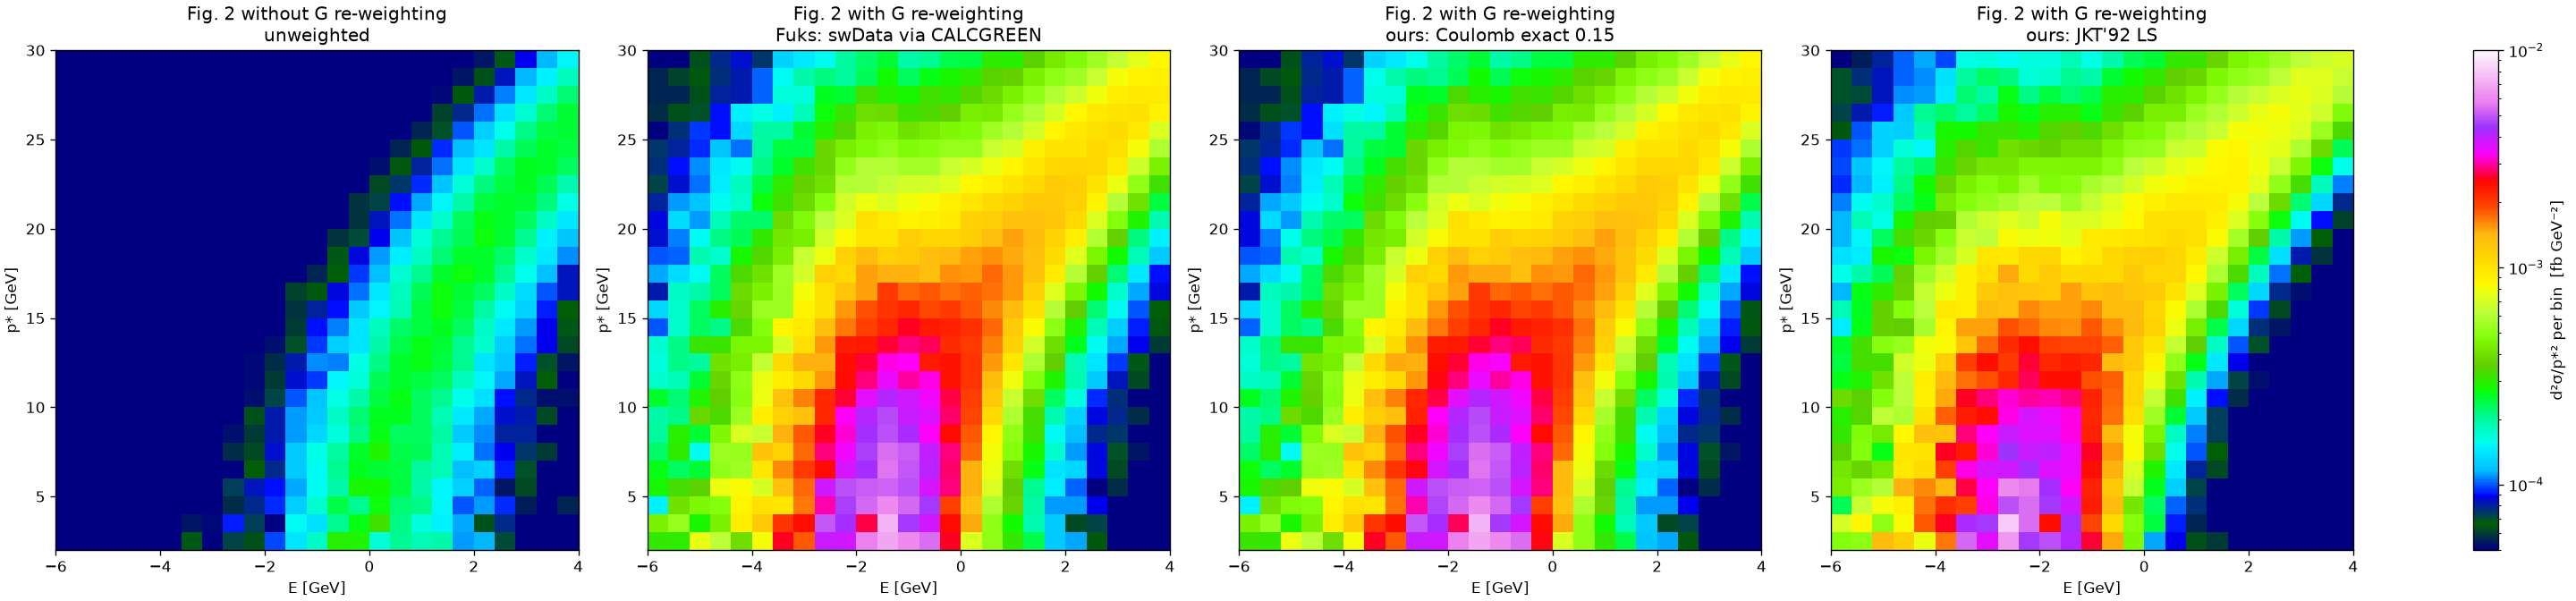
\includegraphics[width=\linewidth]{results/4_fuks_figs2to5/fig2.png}
\caption{Fuks's Fig.~2 from our events: $d^2\sigma/p^{*2}$ per bin in the $(E,p^*)$ plane, without re-weighting and
re-weighted with Fuks's $G$, exact Coulomb at $\alpha=0.15$, and the JKT potential.
(\code{4\_fuks\_figs2to5.py})}
\label{fig:fuks2}
\end{figure}

\begin{figure}[htbp]
\centering
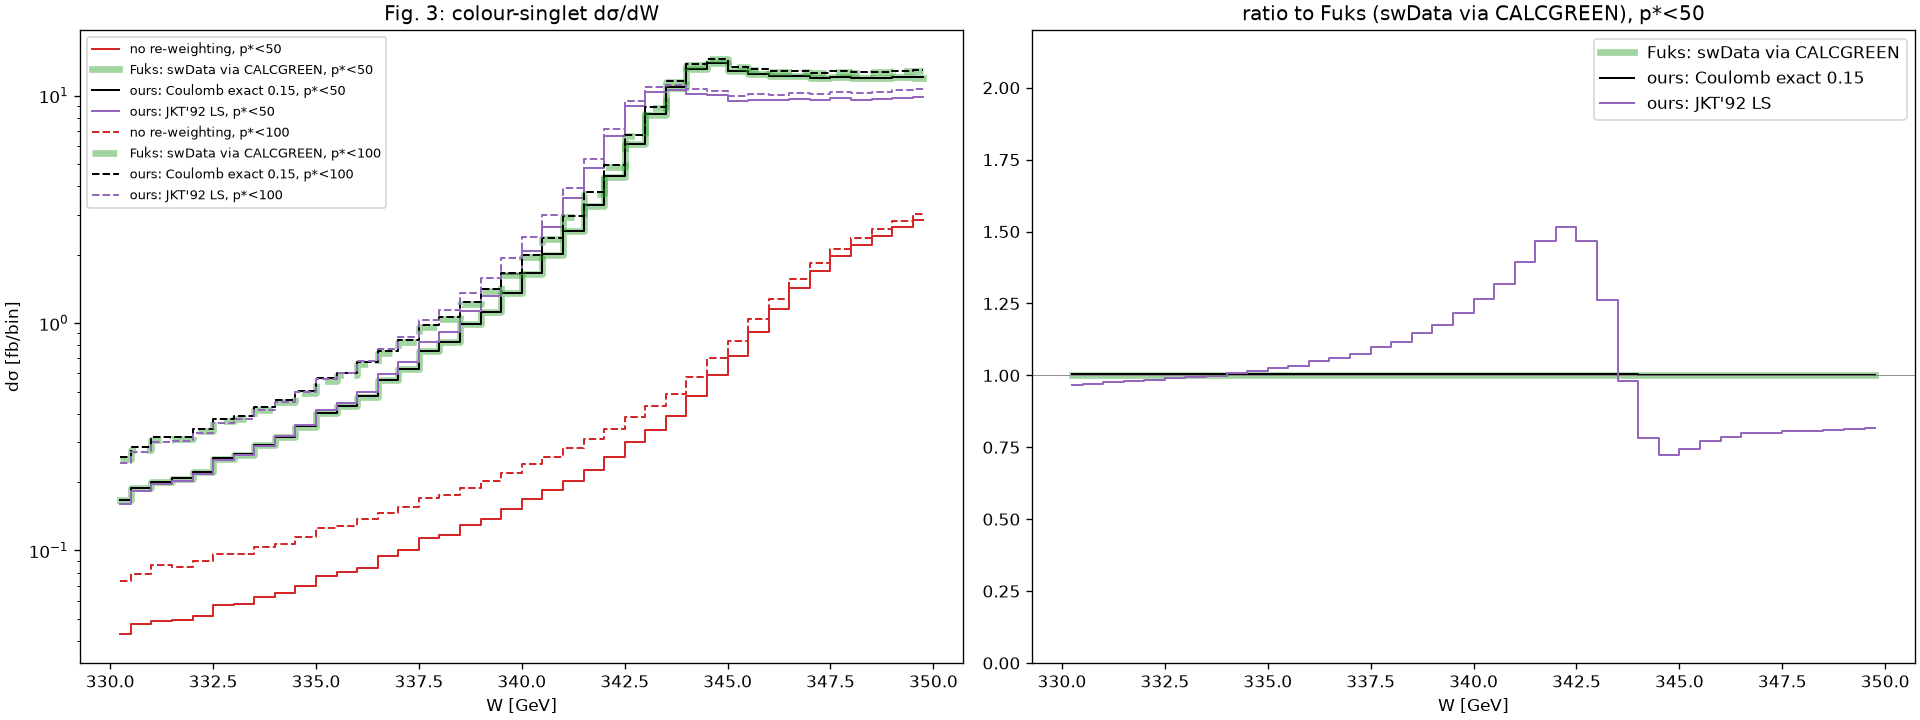
\includegraphics[width=\linewidth]{results/4_fuks_figs2to5/fig3.png}
\caption{Fuks's Fig.~3: colour-singlet $d\sigma/dW$ in 0.5~GeV bins, without re-weighting and re-weighted with the three
sources of $G$, for $p^*<50$ and $p^*<100$~GeV; right, the ratio to Fuks's own $G$. Exact Coulomb at $\alpha=0.15$ lies on
top of Fuks; the JKT potential moves the peak down by about 1~GeV.}
\label{fig:fuks3}
\end{figure}

\begin{figure}[htbp]
\centering
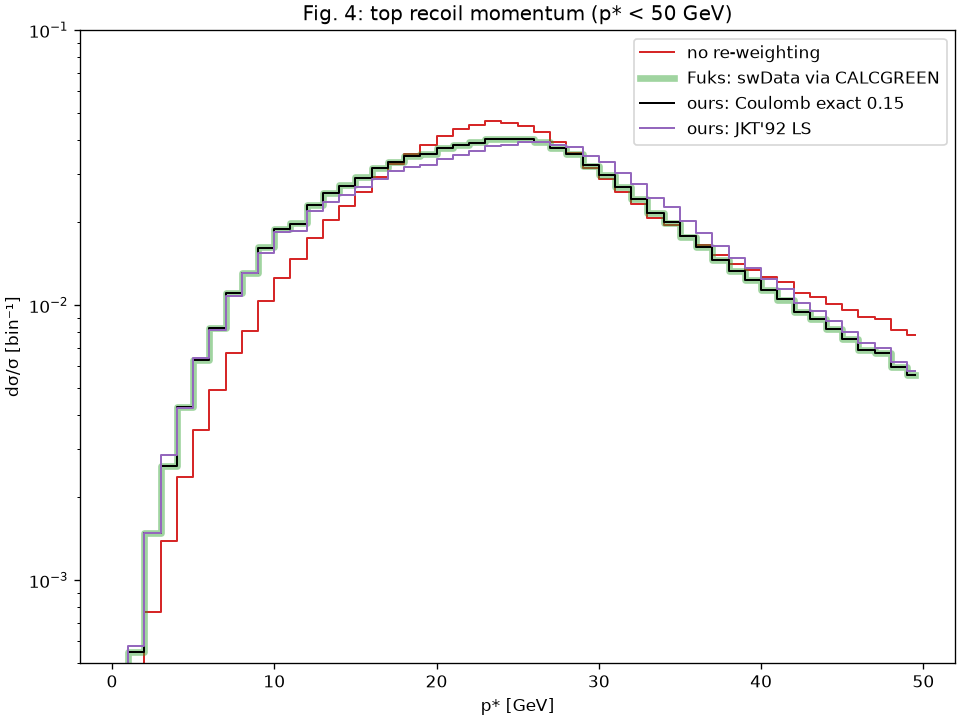
\includegraphics[width=0.55\linewidth]{results/4_fuks_figs2to5/fig4.png}
\caption{Fuks's Fig.~4: the distribution of the top recoil momentum $p^*$ ($p^*<50$~GeV, fraction per 1~GeV bin), without
re-weighting and re-weighted with the three sources of $G$.}
\label{fig:fuks4}
\end{figure}

\begin{figure}[htbp]
\centering
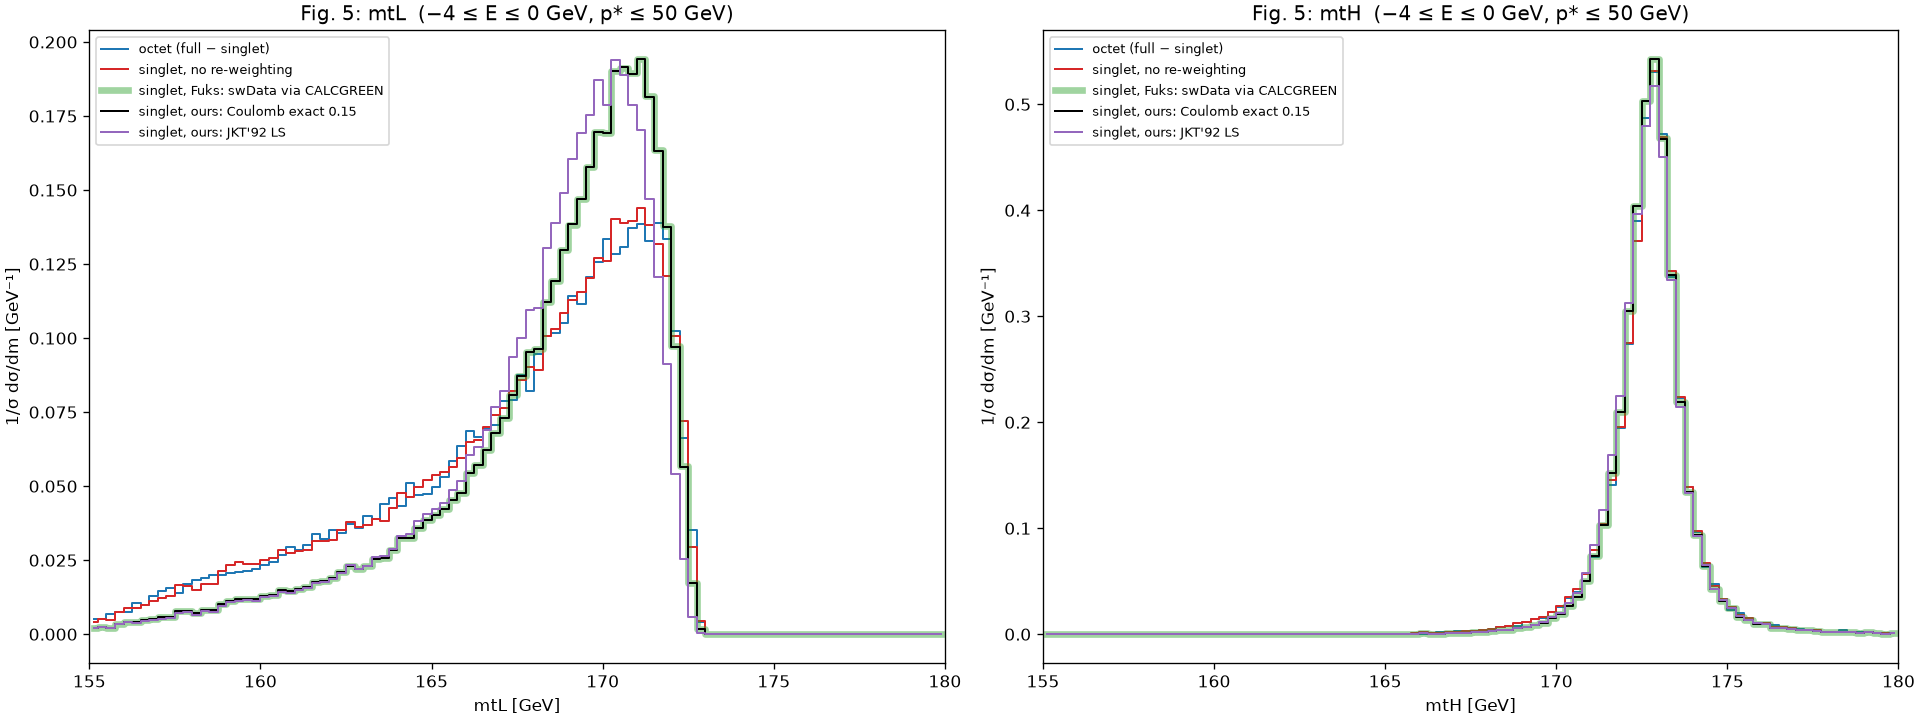
\includegraphics[width=\linewidth]{results/4_fuks_figs2to5/fig5.png}
\caption{Fuks's Fig.~5: the lighter and heavier reconstructed top mass, $m_{t_L}$ and $m_{t_H}$, for $-4\le E\le0$~GeV and
$p^*\le50$~GeV: colour octet, singlet without re-weighting, and singlet re-weighted with the three sources of $G$.}
\label{fig:fuks5}
\end{figure}

%==========================================================================================
\section{Where I fill in or depart from JKT}
\label{sec:departures}
\begin{enumerate}
  \item $\alphas$ is specified at $m_Z$ and $\Lambda_{\MS}$ obtained by solving (14) there; JKT quote $\alphas$ directly.
  \item Grid: JKT's subintervals split once more, at 4 and 60~GeV (Step~5).
  \item $\As(p)$ on a graded auxiliary Gauss--Legendre rule (Step~4); JKT only say ``numerical integration''.
  \item $K$ between the nodes by cubic-spline interpolation (Step~7); JKT do not say how they evaluate off the grid.
\end{enumerate}
Everything else (the potential, the cut and its normalisation, the subtraction, the linear system) is \JKT\ as printed.

%==========================================================================================
\appendix
\section{The code, file by file}
\label{sec:files}
\begingroup\sloppy

Everything lives flat in \code{toponium\_study/}. \code{toponium.py} is the only library; \code{0\_}\ldots\code{5\_*.py} are the
six scripts you run (\code{uv run python 0\_solver\_checks.py}, and so on), each writing \code{results/<stage>/summary.txt} and
figures. Every class opens with an ``EQUATION MAP'' listing which paper equation each method implements.

\subsection*{\code{toponium.py}: six classes, top to bottom}
\begin{description}[style=nextline,leftmargin=1.2em]
\item[\code{Constants}] $m_t$, $\Gt$, $C_F$, $n_F$, and $G_0$, \JKT\ (6).
\item[\code{JKTPotential}] Sec.~\ref{sec:potential}: \code{alpha\_2loop}, \code{lambda\_msbar\_2loop} (14); \code{V\_pert} (13);
  \code{V\_ir}, \code{continuity\_constant\_C}, \code{V\_jkt} (15); \code{V\_cut} (19); \code{V\_cut\_position}, \code{energy\_shift} (20).
  \code{JKTPotential.coulomb(alpha)} gives fixed-coupling Coulomb with the same interface, to test the solver.
\item[\code{LSSolver}] Sec.~\ref{sec:solver}: \code{kernel} (18), \code{jkt\_grid} (23), \code{script\_A} (22), \code{solve\_K} (21),
  \code{G} (16). Usage: \code{LSSolver(potential).G(E, p)}.
\item[\code{CoulombExact}] Sec.~\ref{sec:coulomb}: the exact Coulomb $G$ (\code{G}, fast; \code{G\_adaptive}, slow reference).
\item[\code{FuksTables}] Fuks's swData and \code{CALCGREEN}, used as-is (reference only; nothing of mine is in it).
\item[\code{Events}] the MadGraph events, read from \code{results/4\_fuks\_figs2to5/\_cache\_*.npz}, and the weight $|G/G_0|^2$ for
  $G$ from any of the above.
\end{description}

\subsection*{The six stage scripts}
{\small\noindent\begin{tabularx}{\linewidth}{@{}lL@{}}
\toprule
script & what it does \\
\midrule
\code{0\_solver\_checks.py} & solver vs exact Coulomb, convergence, $\qc$ independence (Sec.~\ref{sec:checks}); \code{kernel\_subtraction.png}\\
\code{1\_validate\_jkt.py} & solver vs JKT's own Figs.~2--5; \code{jkt\_figs.png}\\
\code{2\_identify\_swdata.py} & which potential is in Fuks's tables (Sec.~\ref{sec:fuks})\\
\code{3\_fuks\_fig1.py} & Fuks's Fig.~1 rebuilt from swData, my $G$ alongside\\
\code{4\_fuks\_figs2to5.py} & events re-weighted with the three sources of $G$. Reads \code{\_cache\_full.npz},
  \code{\_cache\_singlet330.npz}: \textbf{the only copy of the events, never delete them}\\
\code{5\_comparison\_tables.py} & CSV tables for comparing with an independent solver (colour singlet): $\Lambda$, $C$, $C_1$,
  $\tilde V_0$ per setting; $\alpha_s(Q^2)$ and each piece of the potential vs $Q^2$; $G$ on $(E,p)$ grids\\
\bottomrule
\end{tabularx}}

\medskip
\noindent \code{reference/} holds both PDFs and swData; \code{README.md} has the recipe to regenerate the MadGraph samples;
\code{pyproject.toml}/\code{uv.lock} define the Python 3.11 environment.
\endgroup

\end{document}
